\section{Désactivation des pare-feu et Windows Defender}

\begin{center}
    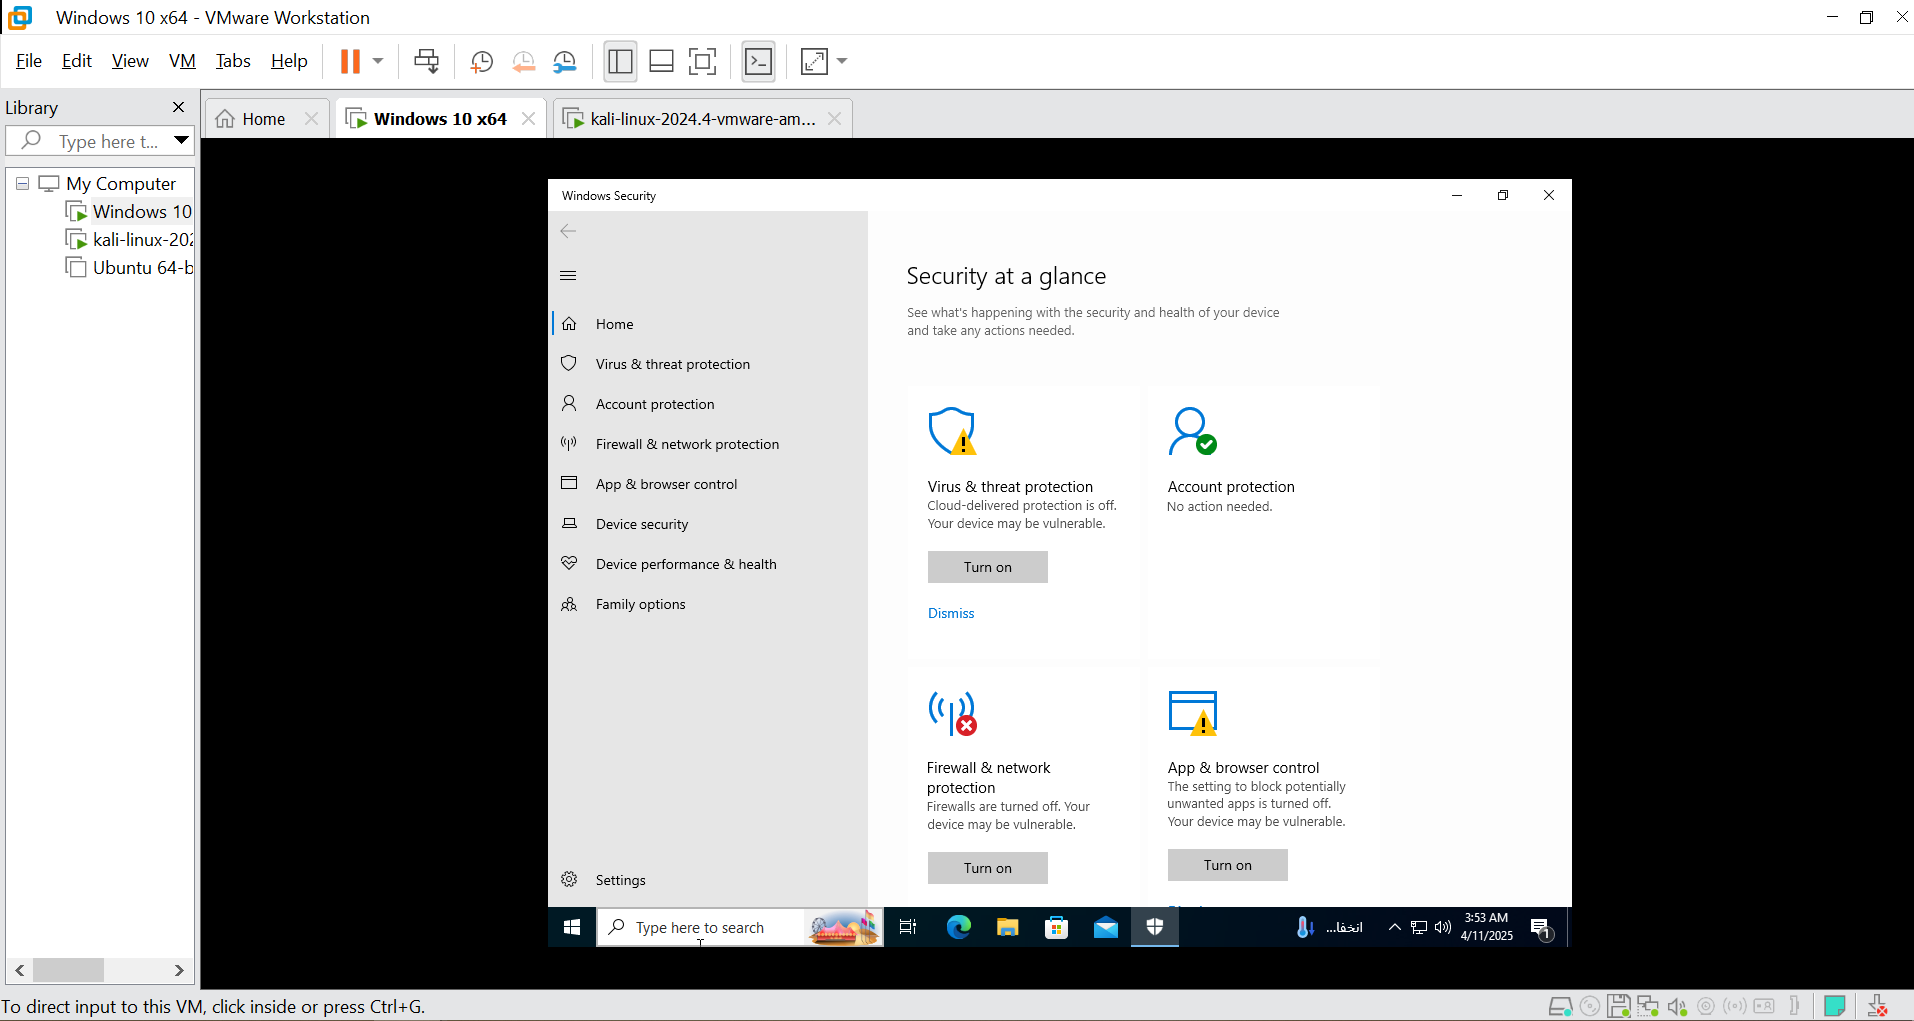
\includegraphics[width=0.8\textwidth]{Question/SC/2-sec.PNG}
\end{center}

\vspace{0.35cm}

\begin{prettyBox}{Pourquoi Les Désactiver}{myblue}
On les désactive parce que Windows Defender détecte les signatures et patterns 
des programmes et virus malveillants, tandis que le pare-feu empêche les communications
non autorisées avec la machine de l'attaquant, qu'elles soient entrantes ou sortantes.
Cette désactivation permet au payload d'exécuter ses actions sans être détecté et
facilite l'établissement d'une connexion reverse TCP entre la machine victime et celle de l'attaquant.
\end{prettyBox}
